\documentclass{article}
\usepackage[a4paper,pdftex]{geometry}

\usepackage[dvips]{graphicx,color,subcaption}
\usepackage{amsmath,amsfonts,amsthm,amssymb,bm} %math stuff
\usepackage{listings,color} %code pasting
\usepackage[utf8]{inputenc} 
\usepackage{authblk}
\usepackage[nottoc,notlof,notlot]{tocbibind} % Put the bibliography in the ToC
\usepackage{siunitx}
\usepackage{setspace}
\usepackage[export]{adjustbox}
\usepackage{booktabs} %references page
\usepackage{textcomp} % provide lots of new symbols
\usepackage{flafter}  % Don't place floats before their definition
\usepackage{natbib} % use author/date bibliographic citations
\usepackage{array} % for better arrays (eg matrices) in maths
\usepackage{paralist} 
\usepackage{verbatim} % adds environment for commenting 
\usepackage{tcolorbox}
\usepackage{multirow}
\usepackage{wrapfig}
\usepackage{pdfpages}
\usepackage{breqn}
\usepackage[section]{placeins}
\usepackage{microtype}
\usepackage{enumitem}
\usepackage{index}
\usepackage{cite}


\begin{document}

\begin{figure}[htp]
    \includegraphics{/Users/austinbenny/Documents/python/movie budget ratings/output/budget_rating.eps}
    \caption{Scheme of the database}
    \label{fig:db}
 \end{figure}

 \begin{figure}[htp]
    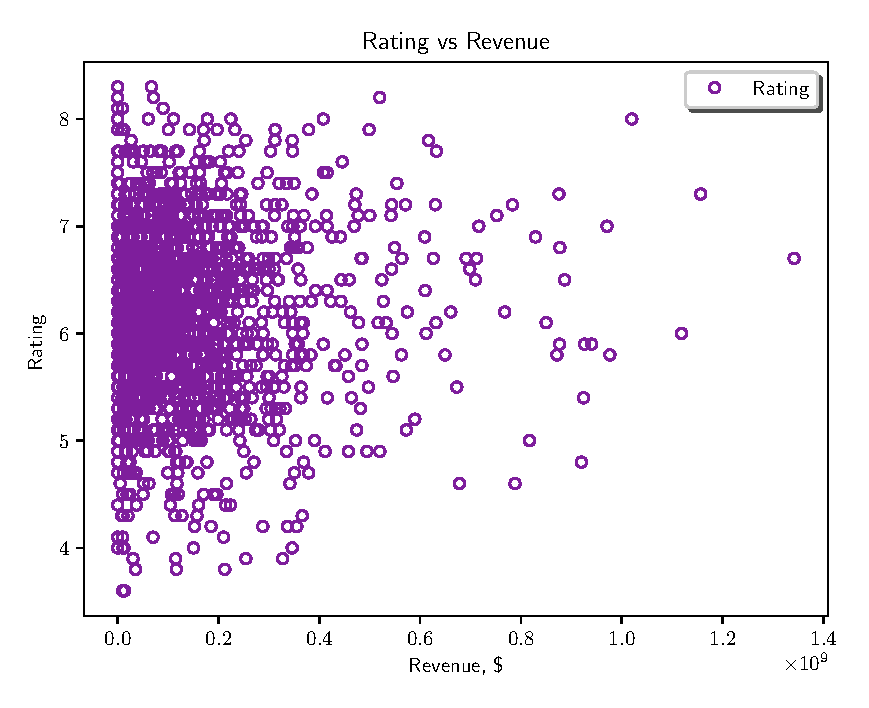
\includegraphics{rating_revenue.eps}
    \caption{Scheme of the database}
    \label{fig:db}
 \end{figure}

 \begin{figure}[htp]
   \includegraphics{budget_rating.eps}
   \caption{Scheme of the database}
   \label{fig:db}
\end{figure}

\begin{figure}[htp]
   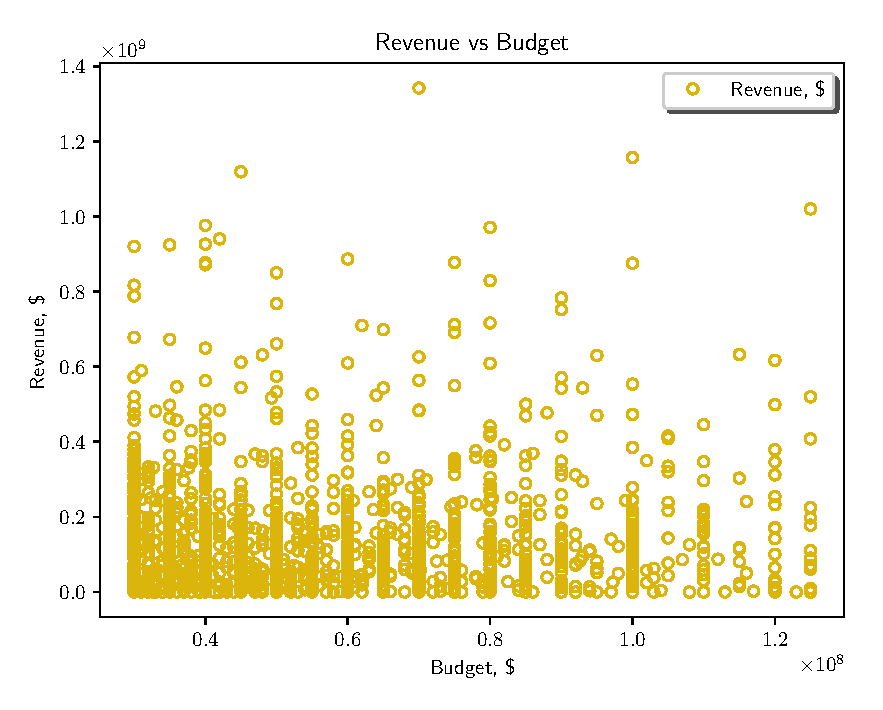
\includegraphics{revenue_budget.eps}
   \caption{Scheme of the database}
   \label{fig:db}
\end{figure}

\end{document}
